% Review: Chris, Aditi, Russell, Yanni, Enbody, Brian Haas, Jared.
% @@spellcheck!
% fix E. coli, de novo.

% Template for PLoS
% Version 1.0 January 2009
%
% To compile to pdf, run:
% latex plos.template
% bibtex plos.template
% latex plos.template
% latex plos.template
% dvipdf plos.template

\documentclass[10pt]{article}

% amsmath package, useful for mathematical formulas
\usepackage{amsmath}
% amssymb package, useful for mathematical symbols
\usepackage{amssymb}

% graphicx package, useful for including eps and pdf graphics
% include graphics with the command \includegraphics
\usepackage{graphicx}

% cite package, to clean up citations in the main text. Do not remove.
\usepackage{cite}

\usepackage{color} 

% Use doublespacing - comment out for single spacing
%\usepackage{setspace} 
%\doublespacing


% Text layout
\topmargin 0.0cm
\oddsidemargin 0.5cm
\evensidemargin 0.5cm
\textwidth 16cm 
\textheight 21cm

% Bold the 'Figure #' in the caption and separate it with a period
% Captions will be left justified
\usepackage[labelfont=bf,labelsep=period,justification=raggedright]{caption}

% Use the PLoS provided bibtex style
\bibliographystyle{plos2009}

% Remove brackets from numbering in List of References
\makeatletter
\renewcommand{\@biblabel}[1]{\quad#1.}
\makeatother


% Leave date blank
\date{}

\pagestyle{myheadings}
%% ** EDIT HERE **


%% ** EDIT HERE **
%% PLEASE INCLUDE ALL MACROS BELOW

%% END MACROS SECTION

\begin{document}

% Title must be 150 characters or less
\begin{flushleft}
{\Large
\textbf{Digital Normalization of Short Shotgun Sequences Facilitates
{\em de novo} Sequence Assembly}
}
% Insert Author names, affiliations and corresponding author email.
\\
C. Titus Brown$^{1,\ast}$, 
Adina Howe$^{2}$,
Qingpeng Zhang$^{3}$,
Alexis B. Pyrkosz$^{4}$,
Timothy H. Brom$^{3}$
\\
\bf{1} Departments of Computer Science and Engineering/Microbiology and Molecular Genetics, Michigan State University, East Lansing, MI, USA
\\
\bf{2} Departments of Microbiology and Molecular Genetics/Crop and Soil Sciences, Michigan State University, East Lansing, MI, USA
\\
\bf{3} Department of Computer Science and Engineering, Michigan State University, East Lansing, MI, USA
\\
{\bf{4} USDA Avian Disease and Oncology Laboratory, East Lansing, MI, USA}
\\
$\ast$ E-mail: Corresponding ctb@msu.edu
\end{flushleft}

% Please keep the abstract between 250 and 300 words
\section*{Abstract}

{\bf Background:} Deep shotgun sequencing and analysis of genomes,
transcriptomes, amplified single-cell genomes, and metagenomes enable
the sensitive investigation of a wide range of biological
phenomena. However, it is increasingly difficult to deal with the volume of data
emerging from deep short-read sequencers, in part because of random
and systematic sampling variation as well as many sequencing errors.
These challenges have led to the development of entire new classes of
short-read mapping tools such as Bowtie and BWA, as well as new de
novo assemblers such as ABySS, Velvet, SOAPdenovo, ALL-PATHS, and SGA.
Even newer assembly strategies for dealing with transcriptomes,
single-cell genomes, and metagenomes have also emerged.  Despite these
advances, algorithms and compute capacity continue to be challenged by
the continuing improvements in sequencing technology.
\\
\\
{\bf Methodology and Principal Findings:} We describe an approach we term
digital normalization, a single-pass computational algorithm that
reduces both sampling variation and the number of errors in deep sequencing data. Digital normalization substantially
reduces the size of data sets and accordingly decreases the memory and time
requirements for {\em de novo} sequence assembly, all without significantly
impacting content of the generated contigs.  Moreover, several data sets
yield a significant improvement in assembly contiguity after digital normalization
is performed.
\\
\\
{\bf Conclusions and Significance:} The digital normalization approach
systematically reduces data set size and removes errors prior to {\em
de novo} sequence assembly.  We demonstrate its
applicability to the assembly of microbial genomes, single-cell
genomic data, and transcriptomic data.

% Please keep the Author Summary between 150 and 200 words
% Use first person. PLoS ONE authors please skip this step. 
% Author Summary not valid for PLoS ONE submissions.   
\section*{Author Summary}

\section*{Introduction}

The ongoing revolution in DNA sequencing technologies has led to a new
problem: how do we analyze the resulting very large sequence data sets
quickly and efficiently? These data sets contain millions to billions
of short reads, and have high error rates and substantial sampling
biases.  The vast quantities of deep sequencing data produced by
these new sequencing technologies are driving
computational biology to extend and adapt previous approaches to sequence
analysis.  In
particular, the widespread use of deep shotgun sequencing on
previously unsequenced genomes, transcriptomes, and metagenomes, has
resulted in the development of several new approaches to de novo
sequence assembly.

There are two basic challenges to dealing with short-read sequences
from shotgun sequencing. The first is that deep sequencing is needed
for thorough sampling. This is because shotgun sequencing samples
randomly from populations of molecules; this sampling is
generally biased by sample content,
sample preparation and sequencing technology, which requires even deeper
sequencing to overcome.  For this reason, a
human genome may require 100x coverage or more for near-complete
sampling, leading to 300 gigabase+ data sets.  Since the minimum sampling depth
is determined by the prevalence of the lowest abundance molecule, transcriptomes and
metagenomes may also require similarly deep sequencing for complete
sampling of rare molecules. This leads to extremely large amounts of
sequencing data.

The second problem with short-read shotgun sequencing is the high
error rate.  Illumina GAII has up to a 1\% error rate in its
sequences, yieldng an average of one base error in every 100 bp of
data.  These errors grow linearly with the amount of data generated and
dominate novelty in high-coverage sequencing data sets.  Tracking this
novelty and resolving errors is computationally expensive.

These two problems have combined to result in a significant
computational challenge: it is now straightforward to generate data
sets that cannot easily be analyzed computationally.  While hardware approaches
to scaling existing algorithms are emergeing, sequencing capacity
is continues to grow faster than computational capacity.
This arms race cannot be won only through improvements
in hardware.  What algorithmic solutions have been applied?

Analysis of the large amounts of data resulting from deep sequencing
has been tackled in a number of ways.  A new class of alignment tools,
mostly relying on the Burroughs-Wheeler transform, has been created
specifically to do ultra-fast short-read alignment to reference
sequence.  In cases where the reference sequence must be assembled de
novo from the sequence data, a number of new assemblers have been
created, including ABySS, Velvet, SOAPdenovo, ALLPATHS, and SGA.
These assemblers rely on theoretical advances such as the application
of de Bruijn graphs and compressed @LM data structures to store large
amounts of data in a computationally convenient manner.  As short-read
sequencing has been applied to single cell genomes, transcriptomes,
and metagenomes, yet another generation of assemblers has emerged to
handle reads from very abundance-biased populations of molecules;
these tools, including Trinity, Oases, MetaVelvet, Meta-IDBA, and
Velvet-SV, adopt local models of sequence coverage to help build
assemblies.  Because these tools all rely on k-mer approaches and
require exact matches between sequences, their performance is
extremely sensitive to the number of errors present in the underlying
data.  This sensitivity to errors has led to a number of error removal
and correction approaches.

Several approaches have been applied to detecting and removing or
correcting errors in large data sets.  Typically, these approaches
involve finding low-abundance fixed-length words, or k-mers, and treating
them as likely errors; these errors can then be eliminated or
``corrected'' by changing them to similar k-mers that are in high
abundance.  One challenge for these techniques is that they
require at least two complete iterations across the data set: one
iteration to count all k-mers, and a second to perform the
trimming or correction.  For extremely large data sets, this
is a significant problem: the ``noise'' from
sequencing errors drives a supra-linear increase in the number of
k-mers, so as data set size increases, the computation and memory
needed to track k-mers increases dramatically.

Here, we describe a single-pass algorithm for detection and
elimination of redundant reads in data sets that provides a method for
reducing data set size and error content, and correspondingly reduces
computational requirements for de novo assembly.  This algorithm, which
we call digital normalization, is inspired by experimental
normalization techniques and was initially designed to deal with reads
from very abundance-biased samples such as single-cell amplified
genomic DNA, transcriptomes, and metagenomes.  Digital normalization
works by systematically removing redundant reads from data sets.
However, by eliminating redundant reads, errors from those reads do
not accumulate in the normalized data set, and we see a
correspondingly substantial reduction in both data size and total
number of errors.  We present a constant-memory implementation of this
approach that operates in time linear with the size of the input data.
We demonstrate its effectiveness for reducing compute requirements
for de novo assembly on several real data sets, including data from a
microbial genome, MDA-amplified single-cell genomic DNA, and a mouse
transcriptome.

% Results and Discussion can be combined.
\section*{Results}

\subsection*{Median k-mer abundance of a read is a good estimator of coverage}

Suppose that we have a file of short reads that are randomly sampled
without error from a non-repetitive source genome, and we want to know
the number of times a specific genomic location is represented in the
reads.  This number, known as the coverage, is typically estimated by
assembling a reference sequence, mapping the short reads back to this
reference, and counting the number of reads that map to the location.
However, this requires assembling a reference sequence, which can be
computationally expensive.  Can we estimate the coverage of a source
genomic region solely from the reads, without having access to a
reference?

One approach to estimating coverage is to select a read overlapping
the location of interest, and then apply the following
procedure. First, choose a $k$ such that k-mers in the single-copy
source genome are unique; a k-mer size of 20 usually serves (cite
k-mer counts paper).  Next, for each k-mer in the selected read,
calculate the number of times that the k-mer appears in {\em any} read
across the entire data set.  The abundance of these k-mers will
represent the true depth of sampling of the source genome for each
k-mer.  We can then estimate the sampling rate or coverage of the
region to which the read belongs by calculating a summary statistic
such as the median or average of the read's k-mer abundance
distribution: see Figure \ref{fig:rankabund}, ``no errors'' line. This
approach relies on the observation that because reads come from a
single location in the genome, the abundances of non-repetitive k-mers
within the read are correlated.  The median provides a measure that
is robust to extreme abundance values stemming from repeats.

We can extend this estimation technique to reads sampled {\em with}
error by observing that each single-base miscall or indel changes no
more than $k$ k-mers in the read (see Figure \ref{fig:rankabund}).  If
the errors are random and $k$ is large, these k-mers will be low
abundance in the read data set.  So, if we order the k-mers in a read
by their abundance across the entire data set, only the abundance of
the first $k$ ranked k-mers will be affected by a single error, and at
most the first $2k$ ranked k-mers will be affected by a pair of
errors.  The median of the k-mer rank-abundance distribution will have
rank $(l - k + 1) / 2$; this is greater than $k$ for $l > 3k-1$, and
greater than $2k$ for $l > 5k-1$.  Thus for read lengths of 76 bases
or longer, and a k-mer size of 20, the median k-mer abundance will
ignore low abundances from a single substitution error; for a read
length of 100, and a k-mer size of 20, the median k-mer abundance will
be robust to two substition errors.

We can therefore use the median k-mer abundance of a read, measured
across the entire read data set, as an estimator of sampling depth for
the region represented by the read. How well does median k-mer
abundance correlate with the abundance calculated from read mapping?
In Figure \ref{fig:random}a, we show that for simulated 100-base reads
from an artificial (non-repetitive) genome of 400kb, sampled with a
1\% per-base error rate, the median 20-mer abundance matches both the
true coverage and the estimated coverage obtained from mapping the
reads back to the genome with bowtie ($r^2 = 0.79$).  Can we apply
this approach to reads from real genomes?

When we apply the median k-mer abundance measure to real reads sampled
from a {\em E. coli} genome, we see the same strong correlation
between median k-mer abundance and estimated coverage based on mapping
\ref{fig:random}b ($r^2=0.80$).

This same correlation also holds for reads sampled from a non-uniform
molecular distribution such as transcriptome or metagenome shotgun
sequencing.  Figure \ref{fig:transcripts}a shows that median k-mer
abundance and number of mapped reads correlate for a simulated
transcriptome with expression across 3 orders of magnitude ($r^2 =
0.93$).  Figure \ref{fig:transcripts}b shows the same strong
correlation for a mouse mRNAseq data set ($r^2 = 0.90$).

\subsection*{The median k-mer abundance can be used to remove redundant reads.}

We can now use the median k-mer abundance to progressively accumulate
only informative (non-redundant) reads, that is, reads that add
significantly to estimated coverage.  Significantly, we can do this
{\em without} a reference sequence.

Suppose we treat the read data set as an incoming stream of data
consisting of reads which we can individually accept or reject.  For
each read, we use the median k-mer abundance to estimate the coverage
of that read based on the reads accumulated so far; if this estimated
coverage is {\em below} a specified threshold, we accept the read, and
otherwise we reject it.  Accepted reads are both saved and
incorporated into the k-mer counts, while rejected reads are simply
discarded.

Algorithmically, we execute the following procedure:

\begin{verbatim}
   for read in dataset:
      if estimated_coverage(read) < C:
         accept(read)
      else:
         discard(read)
\end{verbatim}

where only accepted reads contribute to the estimated coverage.  For
any data set, this has the effect of discarding the majority of reads
that contribute to coverage $>$ C, although overlapping reads may be
accepted later on that push the estimated coverage of earlier reads
above C.  Novel reads -- reads from undersampled regions, or those
reads containing many errors -- will always be retained.

In Figure \ref{fig:coverage}, we display the estimated coverage of a
simulated genome and an {\em E. coli} genome for both raw and
normalized data, using read multimapping (calc @stddev).  From this,
we see that digitally normalizing both simulated and real
high-coverage data has the expected effect of normalizing the
estimated coverage of the reads to C, not only for median k-mer
abundance but for read multimapping.  For both simulated and real
data, then, digital normalization downsamples the data set to only a
subset of reads -- those reads that contribute to additional coverage
below a certain threshold.  Digital normalization thus converts {\em
  high random sampling} to {\em low systematic sampling}.

At what rate are informative sequences retained?  For the E. coli data
set, Figure \ref{fig:accumulate} shows the rate of retention of
sequences against the total number of reads examined for normalizing
to C=20 at k=20.  There is a clear saturation effect showing as more
reads are examined, a smaller fraction of reads are retained; by 5m
reads or approximately 100x coverage of {\em E. coli}, under 30\% of
new reads are kept.  This demonstrates that only a very small amount
of novelty (in the form of either new information, or the accumulation
of significant errors) is being observed as sequencing depth increases.

\subsection*{Digital normalization removes many sequencing errors}

The per-base error rate of most next-generation sequencing technologies
is rather high, approaching 1-2\%.  
These
errors dramatically affect the total number of k-mers; for example, in the
simulated genomic data of @200x, a 1\% error rate leads to more than
20-fold more 20-mers in the reads than are truly present in the genome,
or approximately 20 new k-mers for each error (Table 1, row 1).
This in turn dramatically increases the memory requirements for
tracking and correcting k-mers (cite bloom filter paper).

When we perform digital normalization on such a data set, we eliminate
the vast majority of these k-mers (Table 1, row 1).  Intuitively, this is
because we are accepting or rejecting individual reads; in going from
200x random coverage to 20x systematic coverage, we are discarding
80\% of the reads containing 62\% of the errors (Table \ref{tab:normC20}, row 1).
For reads taken from a biased abundance distribution, such as with
mRNAseq, we also discard many reads, and hence many errors (Table \ref{tab:normC20}, row 2).
Conveniently, in doing so we retain nearly all real k-mers.

During the initial data set reduction we also count the k-mers in the
accepted reads.  With this information we can execute a second pass
across the accepted reads in which we trim reads at low-abundance
k-mers, thus removing another set of likely errors.  Following this
second pass error reduction, we may also execute a second round of
digital normalization that further eliminates redundant data; this
three-pass protocol eliminates some additional errors, at the cost
of very few real k-mers (Table \ref{tab:normC5}).  Because the first
pass discards substantial amounts of data as well as many erroneous
k-mers, later passes are very fast.
% @CTB put my argument to Adina in here.

Interestingly, our three-pass protocol removed many more real k-mers
from the simulated mRNAseq data than from the simulated genome (351 of
48,100 true (0.7\%) lost in the mRNAseq, vs 4 of 399,981 lost
(.000001\%)).  While still only a tiny fraction of the total number of
real k-mers, the difference is striking -- the simulated mRNAseq lost
k-mers at almost 1000-fold the rate of the genomic!  Upon further
investigation, {\em all} of the lost k-mers were located near to the
ends of the source sequences; see Figure \ref{fig:suppleEnd}.  This is
because digital normalization cannot distinguish between erroneous
k-mers and k-mers that are undersampled due to edge effects.  In the
case of the simulated genome, which was generated as one large
chromosome, the effect is negligible, but the simulated transcriptome
was generated as 100 transcripts of length 500.  This presents much
more opportunity for real information loss.

\subsection*{Digital normalization facilitates de novo assembly of genomic data}

We applied the three-pass digital normalization and error trimming
protocol to several real data sets prior to assembly, including
sequences from high-coverage single colonies and a single-cell
MDA-amplified genome.  We then ran the Velvet de novo assembler on the
resulting reads to generate contigs, and compared the sequence content
of the resulting assemblies to the best known reference (see Methods).
In all cases, digital normalization discarded well over 90\% of the
reads as redundant, while the resulting assemblies were over 95\%
identical to the known reference.

@@

@Do we need to look at mapped reads after assembly to verify uniformity
of coverage?

\subsection*{Digital normalization facilitates de novo assembly of transcriptomes}

We next applied single-pass digital normalization to a published mouse
mRNAseq data set, reducing it to a maximum of 20x coverage for k=20,
and assembled both the original and normalized sequence reads with
Oases and Trinity, two de novo transcriptome assemblers.

@@

In both cases the computational resources necessary to complete an
assembly were significantly reduced (Table \ref{tab:dntrans}), but
normalization had different effects on the assemblers.  In the case of
the Trinity assembly, both the number of transcripts greater than 300
bases and the sum total of bases in transcripts greater than 300 bases
were severely affected by digital normalization.  We used BLASTN to
compare sequence content at a length of 200 bases, and determined that
while 99.0\% of the sequence in the normalized Trinity assembly mapped
to the full Trinity assembly, only 85.6\% of the full Trinity assembly
mapped to the normalized Trinity assembly.  Thus a significant portion
of long regions in the full transcriptome was lost after digital
normalization.  However, 98.4\% of the unique 26-mers in the full
Trinity assembly were found in the normalized Trinity assembly, so the
core sequence content was not that different.

(@CTB mention BLAST multi align; see Trinity
paper for their method.)

In contrast, while the number and sum total of bases were reduced in
the normalized Oases assembly, 98.6\% of the normalized Oases
assembly mapped to the full Oases assembly, and 98.5\% of the full
Oases assembly mapped to the normalized assembly -- suggesting that
the assemblies were virtually identical in terms of sequence content.
One explanation for this loss is that digital normalization
eliminated low-abundance splice variants, while retaining the
individual exons.

(@CTB how do we confirm?  blast comparison of isoforms is bridging splice connex?)

There are two possible reasons for the substantial negative effect of
digital normalization on the Trinity assembly.  First, digital
normalization could be eliminating k-mers that are used in the
assembly; and second, digital normalization could be affecting the
Trinity algorithm for determining likely transcripts.  To further
investigate the Trinity results, we adopted the ``Oracle set''
approach used in Grabherr et al. (2011) and examined the extent to
which k-mers in the original and normalized data set covered the full
Trinity assembly XXXπ.  We found that all but 0.5\% of the k-mers used in
the Trinity assembly were present in the normalized assembly.
Furthermore, all of the lost k-mers were at the ends of the
reconstructed transcripts, suggesting that the end-sampling bias
observed with the simulated data (above) was the source of this minor loss.
Together with the Oases results, this suggests that there is no
inherent and substantial loss of informative k-mers because of digital
normalization.  This implies that digital normalization is primarily
affecting the algorithm that Trinity uses to determine which reads to
assemble into transcripts.

% @CTB change-k-value argument? what if we could change k value for trin?

@@ do we want to do a SICB-like image of read mapping / redundancy?

\section*{Discussion}

\subsection*{Digital normalization discards redundant data and removes errors}

Digital normalization is a simple, lightweight computational technique
for removing redundant data from shotgun sequencing data sets.
Digital normalization is similar in concept to experimental
normalization, which has been used for sequencing both mRNA and
single-cell amplified genomes, but it is applied computionally --
after sequencing.  In contrast to experimental normalization, digital
normalization still requires deep sequencing to sample rare molecules;
however, digital normalization confers several advantages over
experimental normalization, including the ability to recover source
molecule abundances from (digitally) discarded reads.

\subsection*{Digital normalization dramatically scales de novo assembly}

The results from applying digital normalization to read data sets
prior to de novo assembly are extremely good: digital normalization
reduces the computational requirements (time and memory) for assembly
considerably, without substantially affecting the assembly results.
Why is this?

First, by discarding reads that do not contribute significant
additional information, digital normalization removes the majority of
reads without affecting the real information content of the read data
set.  For de Bruijn graph assemblers such as Velvet, this reduces the
storage requirements for loading and tracking reads.

Second, by discarding the majority of reads from deep sequencing data
sets, digital normalization eliminates sequencing errors contained in
those reads.  These sequencing errors add significantly to memory
usage for assemblers like Velvet, so eliminating them reduces the
memory required for assembly.

Third, by converting random sampling to systematic sampling and
normalizing the coverage, digital normalization corrects bias in read
coverage, including that due to sampling bias and underlying
non-uniform molecule distributions.  This allows single-genome
assemblers such as Velvet to be applied to sequences from samples with
biased source distributions such as mRNAseq and MDA-amplified genomes,
as well as metagenomic samples from mixed-abundance populations,
without modification.

Fourth, digital normalization is directly congruent to the de Bruijn
graph approach used in many modern assemblers.  Because de Bruijn
graph assemblers use k-mer connectivity to build contigs, and k-mer
novelty is used by digital normalization as the criterion for
retaining a read, the graph structure should not be not changed
significantly by normalization.  Thus we believe that digital
normalization will be a generally effective approach for preprocessing
data for {\em any} de Bruijn graph assembler.  Demonstrating this
remains for future work, as does a study of precisely what parameters
perform best with which assemblers.

@@show figure of converted coverage from nonuniform distribution!

The net effect of digital normalization is to significantly reduce
computational requirements for {\em de novo} assembly.  This is not a
trivial consideration: as stated in Salzberg et al., 2011, ``the
ability to actually complete assemblies is underappreciated. @@'' As
data quantity from next-generation sequencing increases, assembly
becomes ever more challenging; the ability to build transcriptomes and
single- cell genomes quickly and effectively in the face of large
quantities of data is important.  Because digital normalization
converts the assembly problem from a computational problem that scales
with the volume of data to a computational problem that scales with
the size of the underlying genome or transcriptome, it provides a
potential long-term solution to the problem of {\em de novo} assembly.
In particular, we note that Oases assembly of the digitally normalized
mouse transcriptome data can now be run in under 60 GB of RAM.
Computers of this size are available through rental ``cloud
computing'' providers such as Amazon, making it possible for
researchers without substantial compute hardware to do transcriptome
assembly for non-model organisms.

@figure out how to make argument here.

\subsection*{Digital normalization removes isoforms and drops terminal k-mers}

@@discuss failure mode

@@retention of errors at a certain point.

\subsection*{Conclusions}

Digital normalization is an effective demonstration of the basic
observation that at most 2x coverage is required to assemble a genome
-- it just has to be {\em systematic} coverage.  Here we have chosen
to normalize samples to 5x, primarily to ensure $>$ 2x systematic
coverage in the face of sequencing errors.  Normalization and assembly
of data is significantly more computationally efficient than assembly
of the raw reads.  Nonetheless, assembly of normalized data results in
nearly identical assemblies for genomic data, and useful if not
completely sensitive assemblies for transcriptomic data.

The method of digital normalization described above relies on a k-mer
based, reference-independent way of measuring the coverage of
individual reads.  Any reference-free progressive approach to
estimating coverage could serve; for example, an alignment-based
approach, in which reads were progressively used to build alignments
with error tolerance, may provide an alternative implementation that
is less sensitive to errors.

Here we have primarily tackled the problem of {\em contig assembly},
because that is the most computationally challenging part of {\em de
  novo} assembly.  Scaffolding, in which contigs are joined together
based on paired-end information, is necessary for generating longer
sequences in repeat-rich genomes.  Because of this, we have only
examined the results of digital normalization on microbial genomes,
which can yield good assemblies even without scaffolding.  However, in
principle there is no reason that digital normalization cannot be
applied to contig generation in eukaryotic genomes; this remains for
future work.

\subsection*{Digital normalization is widely applicable and computationally convenient}

Digital normalization uses a reference-independent estimator of
coverage, so it can be applied de novo to {\em any} data set.  The
approach is extremely computationally convenient: the runtime
complexity is linear with respect to the data size, and perhaps more
importantly it is {\em single-pass}: the algorithm does not need to
look at any read more than once.  Moreover, because reads are
accumulated sub-linearly, errors do not accumulate and overall memory
usage for digital normalization itself consequently limited.

The first pass of digital normalization is an online streaming
algorithm in which data is examined only once, and information about
the data generally accumulates more slowly than the size of the data
examined.  Streaming algorithms are very useful for solving Big Data
problems in which generated data cannot easily be transmitted,
computed upon, or stored.  Here, we implement a streaming algorithm
using a constant memory data ``sketch'' data structure, CountMin
Sketch.  By combining a single-pass algorithm with a constant-memory
data structure, we provide solution to sequence data analysis with
both (linear) time and (constant) memory guarantees. Moreover, because
the failure mode of the CountMin Sketch data structure is well
understood and easy to examine, we can provide {\em data quality
guarantees} as well.  These kinds of guarantees are immensely
valuable from an algorithmic perspective, because they provide a
robust foundation for further work.

We note that the general concept of removing redundant data while
retaining most information has very broad applicability, especially if
done in a computationally convenient manner.  For example, digital
normalization can be done prior to homology search on unassembled
reads, potentially reducing the computational requirements for
e.g. BLAST and HMMER without loss of sensitivity.  Digital
normalization can also be applied to multiple different read data sets
potentially from different read technologies in order to preferentially
select sequences containing ``new'' information.  These approaches
remain to be explored in future work.

\section*{Leftover text}

\subsection*{Digital normalization can fail}

For what data sets would we expect this correlation between median
k-mer abundance and ``true'' read coverage to break down?

One biological situation in which we would expect to see divergence
between median k-mer abundance and actual read coverage is for a
highly polymorphic diploid or polyploid sequence, or, more generally,
from a population of molecules with a high rate of internal sequence
variation.  This is because k-mers are notoriously sensitive to high
rates of true variation: for k=20, a diploid sequence with a 5\%
polymorphism rate would generate more than half again as many unique
20-mers as were in a haploid sequence.

Another biological situation is that of repetitive sequence or splice
variants, in which many source molecules will contain many identical
k-mers, resulting in reads that cannot resolve true novelty from errors.  When an accurate reference sequence set is available and the
data set is uniformly sampled (e.g. for genome sequencing) it is
straightforward to correct for k-mers that occur multiple times in the
source molecules, by simply averaging each k-mer's counts in the reads
over the actual number of times the k-mer occurs in the reference data
set.  However, this approach has two limitations: first, it cannot be
used in the absence of a high-quality reference sequence; and second,
it cannot be applied when the source data set has a biased abundance
distribution, for example in transcriptomes.

\subsection*{Digital normalization and assemblers}

One concern with digital normalization is that even without any
explicit information loss in terms of real k-mer content, digital
normalization might adversely affect genome assembler heuristics for
dealing with standard genomic features such as repeats.  For example,
Velvet uses k-mer abundance to detect and resolve issues with repeat
traversal.  Digital normalization eliminates the majority of
repetitive k-mers and hence might drive misassembly. Our results above
suggest that at least in microbial genomes, this does not occur
systematically.  This might be because repeats affect assembly less in
microbial genomes than in repeat-rich eukaryotic genomes; we are
currently working to apply digital normalization to contig assembly in
eukaryotic genomes, but this is future work.

Our results from Trinity and Oases suggest that current transcriptome
assemblers are either very sensitive (Trinity) or somewhat sensitive
(Oases) to the effects of digital normalization.  It may be possible
to recover the majority of lost transcripts by altering internal
parameters of the Trinity algorithms, although it is likely that some
low-prevalence isoforms are simply lost in the process of digital
normalization (@@).  Regardless, digital normalization may provide
a sufficiently significant advantage to consider adapting the Trinity
and Oases algorithms to better handle normalized data.

Digital normalization with k-mers may be particularly well-suited to
preprocessing sequences before de Bruijn graph assembly.  Digital
normalization should not significantly change the paths available in
the de Bruijn graph.  In particular, results show that even when the
final assemblies differ, as with Trinity, the k-mers necessary to
reconstruct much of the assembly remain in the data set.

%Discuss fail: repeats, isoforms. Can we construct a fail data set? Has
%to be both repeats and biased abundance.  Correct for # of k-mers.

\subsection*{Future challenges}

The two obvious failure modes for digital normalization -- situations
in which the median k-mer abundance will not match true coverage --
are high polymorphism rates and samples with repetitive sequences,
including splice variants.  These are essentially opposite sides of
same coin: polymorphism will result in coverage estimates that are too
low, while repetitive sequence will result in coverage estimates that
are too high.

In practice, there are a number of practical solutions for sequences
from samples with a high rate of polymorphism, depending on the
analysis goals and the underlying biology.

If the end analysis goal is to provide a single reference sequence via
de novo assembly -- a notoriously challenging assembly problem -- it
should be possible to adapt k-mer based read-correction techniques to
such data, and digital normalization could be used as an initial data
reduction step.

If the end analysis goal is to provide the sequence of all strains or
haplotypes via de novo assembly -- also extremely challenging -- some
effective approaches have been demonstrated in the field of
metagenomics.

Repeats are likely to be a more significant problem, because they are
preferentially eliminated by digital normalization.  This results in a
significant underrepresentation of repeats in the normalized read data
set, and may also confuse assemblers that rely on k-mer abundance to
locate repeats.  In this work, we have avoided analyzing or assembling
highly repetitive genomes.  Generally, effective resolution of repeats
usually requires paired-end sequences from several libraries with
different insert sizes, which we do not have for any of the data sets
analyzed here.  For now, we note that our assembly results compare
well with assembler results on non-normalized data, suggesting that
the effect of digital normalization is minimal on the assembly of
short-insert libraries.

The effect on isoforms is undetermined.  @@  Further work!

@@CTB: rearrange to conclusions, future work; make brief.

\subsection*{Misc foo}

Connections to compressed sensing, loss compression prior to assembly.

Can quantitate off of discarded data.

%Ref to experimental normalization

%The original data set can be retained for quantification against the
%assembled data set.

%repeats, scaffolds

%Talk about normalization helping basic assemblers.

missassembly analysis/a5
a5 refs

NOT just error removal: smooths things out.

stress preprocessing; attacks de Bruijn principles.

ht size scales with original genome size

show graph of accumulation of reads and errors for simulated data set

show graph of accumulation of reads vs new k-mers - linear??

show graph of read/kmer rank abundance

grain of sand foo.

%error correction and/or alignment and/or graph foo

track memory, time

longer sequences

alexis:

Some mappers pride themselves on using base quality scoring.  Might be
necessary to say something about it and why your method doesn't use or
doesn't need to use it.

What about those groups that make mappers who try to claim that
distributing the reads (or in this case kmers) either randomly or
through some statistical weighting will solve the multi position read
problem?  Might need to be mentioned even if only to throw it out.

Possible fail data set: a group of isoforms that collectively have no
unique kmers and are expressed at drastically different levels.  Might
not even need random sampling and errors.

Exon1Exon2Exon3 (10)
Exon2Exon3                (100)
Exon1Exon2             (1000)

In the case where two regions are represented as AXXXB and CXXXD: the
median might start getting screwy when XXX will generate more kmers
than AXX + XXB.  Say AXX generates 50 kmers, then XXX is long enough
to generate 101 kmers, then XXB generates 50 kmers.  The AXX and XXB
kmers are unique to the dataset.  XXX is shared.  All unique kmers
will be eliminated along with all but one shared kmer.

Adina:

They are clearly related, because even if you actually hit each region
(say) five times or more, in a big enough genome there will be some
unlucky region where four of the sampled reads have errors in them,
leaving a *genuine* k-mer (one that is actually in the genome) with an
abundance of 1. Then if we remove abund=1 k-mers, we lose true data.

And if you downsample the data to an average coverage of five, and
*then* trim, you're exacerbating this situation artificially by
choosing only five reads to represent each region, which will then be
more likely to have errors.

If you downsample to 20, then trim, then
downsample again to 5, you're bypassing this problem, by first doing
relaxed data reduction, then error trimming, and then more severe data
reduction again; basically, more scalable error trimming before the
most severe round of data reduction.

Talk about foo.

% You may title this section "Methods" or "Models". 
% "Models" is not a valid title for PLoS ONE authors. However, PLoS ONE
% authors may use "Analysis" 
\section*{Materials and Methods}

% Do NOT remove this, even if you are not including acknowledgments
\section*{Acknowledgments}

Chris Hart, James M. Tiedje, USDA * 2, NSF, Brian Haas.

%\section*{References}
% The bibtex filename
\bibliography{template}

\newpage

\section*{Figure Legends}

\begin{figure}
\centerline{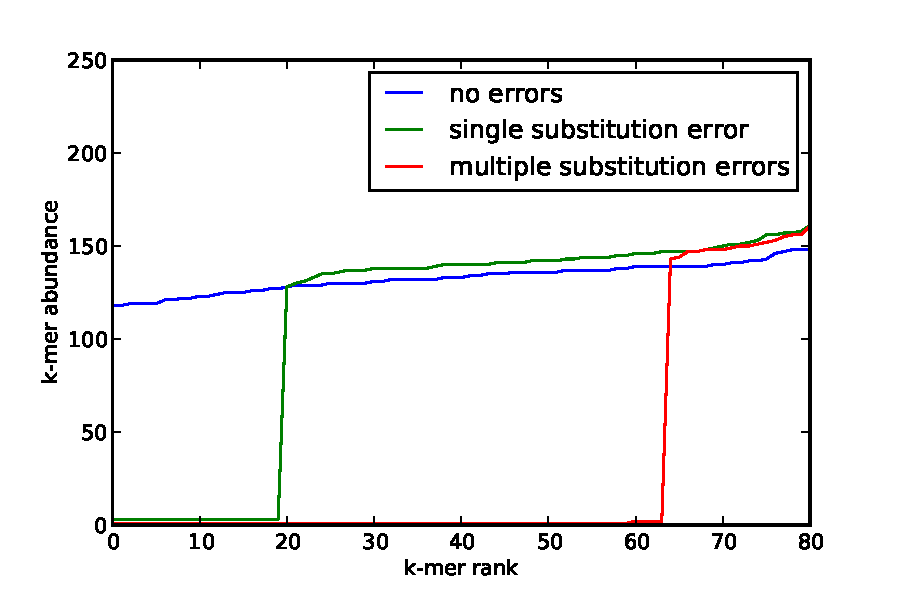
\includegraphics[width=4in]{diginorm-ranks.pdf}}
\caption{
{\bf Representative rank-abundance distributions for k-mers from a read with no errors,
a read with a single substitution error, and a read with multiple
substitution errors.}}
\label{fig:rankabund}
\end{figure}

\begin{figure}[!ht]
\begin{center}
\centerline{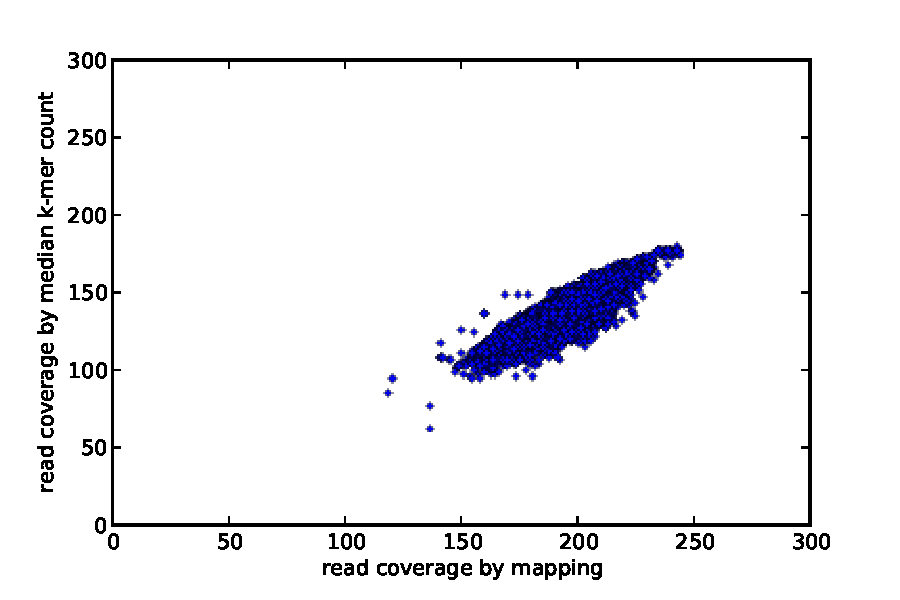
\includegraphics[width=4in]{diginorm-sim-genome.pdf}}
\centerline{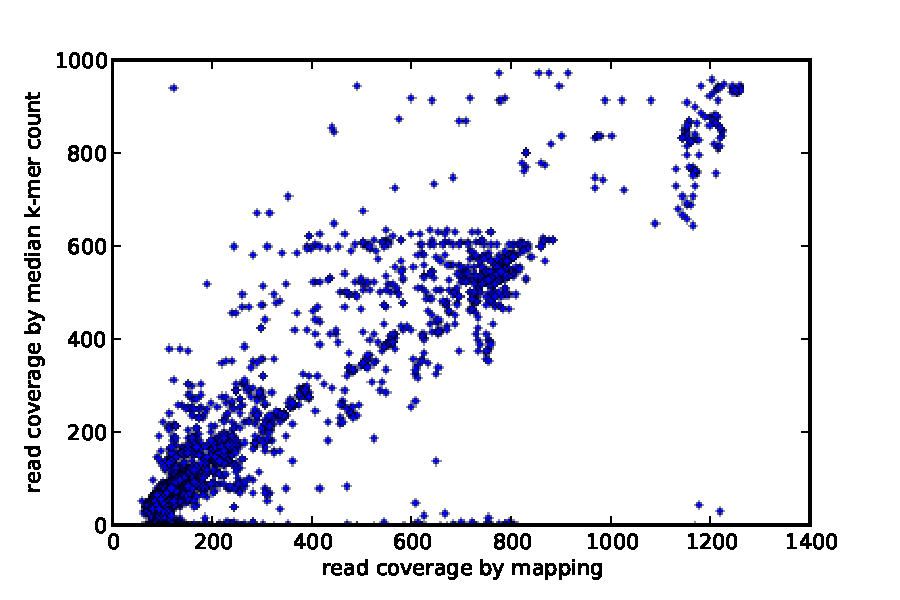
\includegraphics[width=4in]{diginorm-ecoli-genome.pdf}}
\end{center}
\caption{
{\bf Mapping and k-mer coverage measures correlate for simulated genome
data and a real {\em E. coli} data set.  Simulated data $r^2 = 0.79$; {\em
E. coli} $r^2 = 0.80$.}
}
\label{fig:random}
\end{figure}

\begin{figure}[!ht]
\begin{center}
\centerline{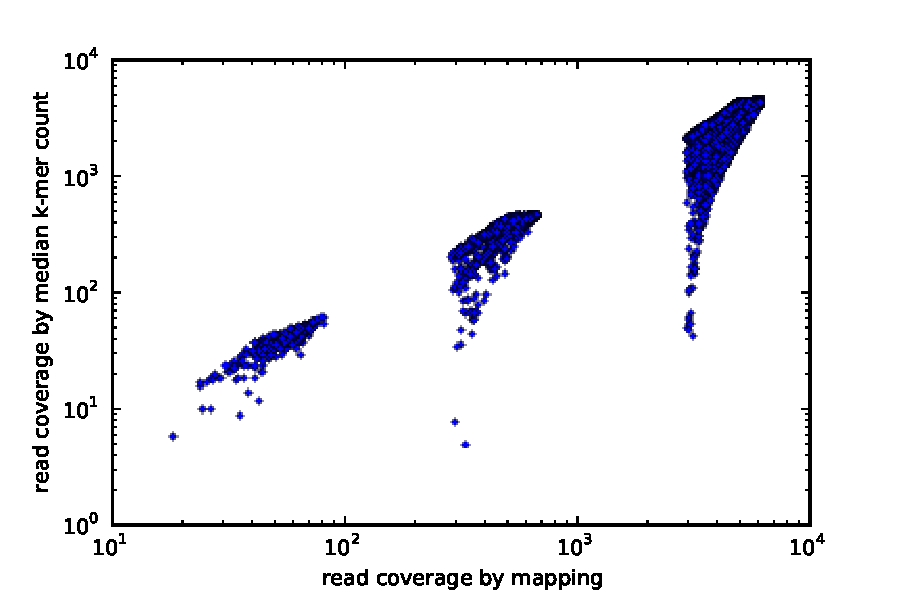
\includegraphics[width=4in]{diginorm-sim-transcr.pdf}}
\centerline{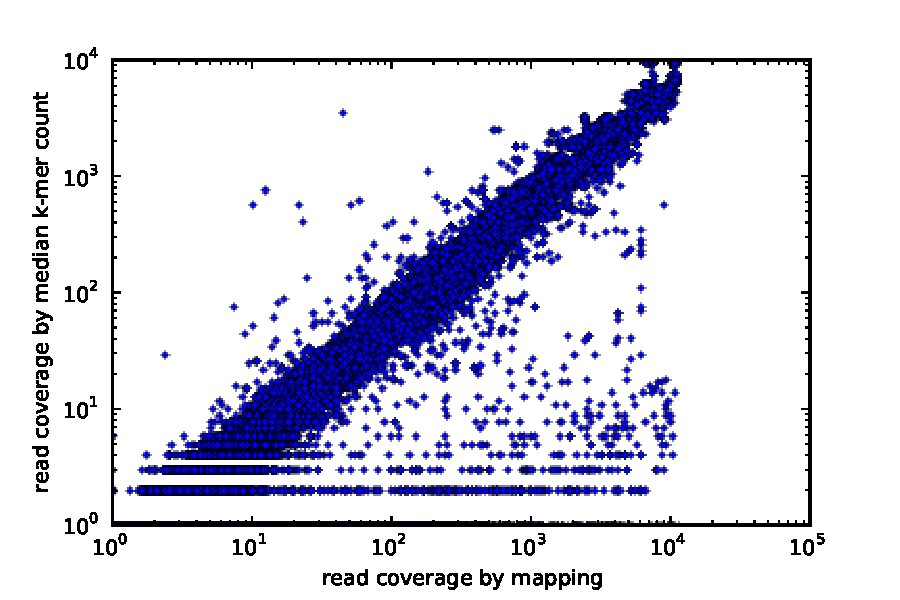
\includegraphics[width=4in]{diginorm-mouse-transcr.pdf}}
\end{center}
\caption{
{\bf Mapping and k-mer coverage measures correlate for simulated transcriptome data as well as real mouse transcriptome data. Simulated data $r^2 = 0.93$;
mouse transcriptome $r^2 = 0.90$.}
}
\label{fig:transcripts}
\end{figure}

\begin{figure}
\centerline{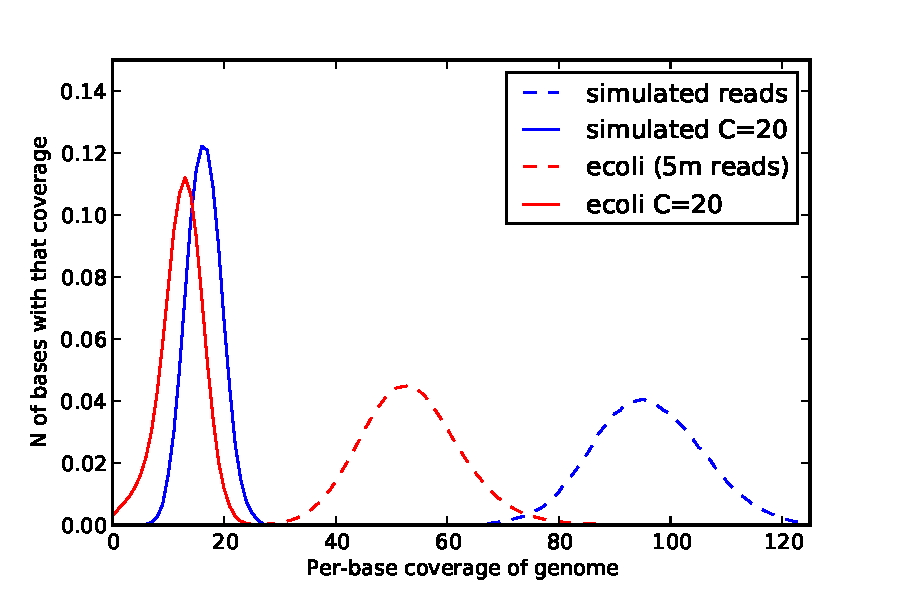
\includegraphics[width=4in]{diginorm-coverage.pdf}}
\caption{
{\bf Coverage distribution of simulated and real genomes, calculated from mapped reads before and after normalization (k=20, C=20).}}
\label{fig:coverage}
\end{figure}

\begin{figure}
\centerline{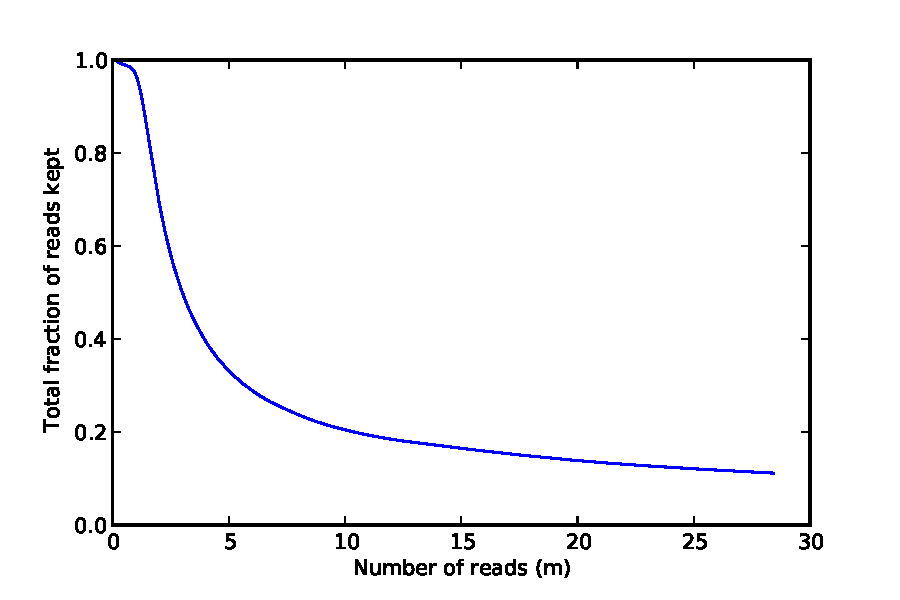
\includegraphics[width=4in]{diginorm-accumulation.pdf}}
\caption{
{\bf Fraction of reads kept when normalizing the {\em E. coli} dataset to C=20 at k=20.}}
\label{fig:accumulate}
\end{figure}

\begin{figure}
\centerline{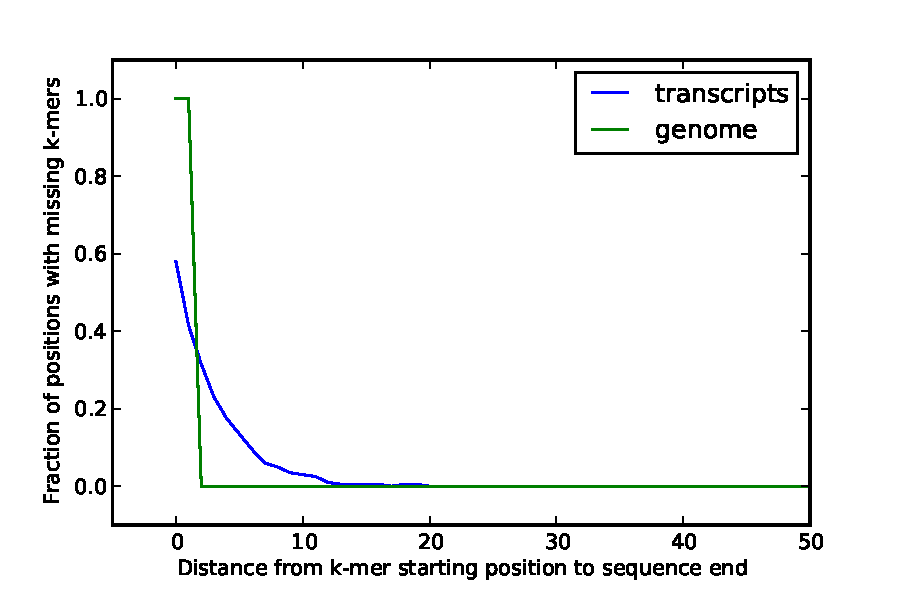
\includegraphics[width=4in]{diginorm-endbias.pdf}}
\caption{
{\bf K-mers at the ends of sequences are lost during digital normalization.}}
\label{fig:supplEnd}
\end{figure}

\section*{Tables}

\begin{table}[!ht]
\caption{
\bf{Digital normalization to C=20 removes many erroneous k-mers from sequencing data sets.  Numbers
in parentheses indicate number of true k-mers lost at each step.}}
\begin{tabular}{|l|c|c|c|c|}
Data set & True 20-mers & 20-mers in reads & 20-mers at C=20 & \% reads kept\\
\hline \\
Simulated genome & 399,981 & 8,162,813 & 3,052,007 (-2) & 19\% \\
Simulated mRNAseq & 48,100 & 2,466,638 (-88) & 1,087,916 (-9) & 4.1\% \\
{\em E. coli} genome & 4,542,150 & 175,627,381 (-152) & 90,844,428 (-5) & 11\% \\
Mouse mRNAseq & XXX & YYY & ZZZ & 28\% \\

\end{tabular}
\begin{flushleft}
\end{flushleft}
\label{tab:normC20}
\end{table}

%%%%%%%%%%%%%%%%%

\begin{table}[!ht]
\caption{
\bf{Three-pass digital normalization removes most erroneous k-mers}}
\begin{tabular}{|l|c|c|c|c|}
Data set & True 20-mers & 20-mers in reads & 20-mers remaining & \% reads kept\\
\hline \\
Simulated genome & 399,981 & 8,162,813 & 453,588 (-4) & 5\% \\
Simulated mRNAseq & 48,100 & 2,466,638 (-88) & 182,855 (-351) & 1.2\% \\
{\em E. coli} genome & 4,542,150 & 175,627,381 (-152) & 7,638,175 (-23) & 2.1\% \\
Mouse mRNAseq & XXX & YYY & ZZZ & AA\% \\
\end{tabular}
\begin{flushleft}
\end{flushleft}
\label{tab:normC5}
\end{table}

%%%%%%%%%%%%%%%%%%

\begin{table}[!ht]
\caption{
\bf{Three-pass digital normalization reduces computational requirements for contig assembly of genomic data.}}
\begin{tabular}{|l|c|c|c|c|}

Data set & Assembly time & Assembly memory & DN assembly time & DN assembly memory \\
\hline \\
{\em E. coli} (5m) & 235s & 2.7gb & 24s & 0.4gb \\
{\em E. coli} (31m) & XXX & YYY & ZZZ & AAA \\
E. coli MDA & XXX & YYY & ZZZ & AAA \\
{\em S. aureus} (XXX) & XXX & YYY & ZZZ & AAA \\
MDA (XXX) & XXX & YYY & ZZZ & AAA \\

\end{tabular}
\begin{flushleft}
\end{flushleft}
\label{tab:dngenome}
\end{table}

%%%%%%%%%%%%%%%%%%%%%%%

\begin{table}[!ht]
\caption{
\bf{Digital normalization reduces computational requirements for assembly of transcriptomic data.}}

\begin{tabular}{|l|c|c|c|c|}

Data set & Assembly time & Assembly memory & DN assembly time & DN assembly memory \\
\hline \\
Mouse (Oases) & XXX & YYY & 73m & 34.6gb \\
Mouse (Trinity) & 2297m & 42.1gb & 634m & 36.4gb \\

\end{tabular}

\begin{flushleft}
\end{flushleft}
\label{tab:dntrans}
\end{table}


\end{document}

